% !TeX spellcheck = en_US
\chapter{Robotics Sensor Systems}
This chapter gives an overview on different types of sensors used in robotic systems, the physics behind them and more \dots

\section{Overview}
Two classes of sensors:
\begin{table}[hbt!]
	\centering
	\begin{tabular}{p{8cm}|p{8cm}}
		Proprioceptive sensors & Exteroceptive sensors \\\hline\hline
		\textit{Proprioception}, also referred to as \textit{kinaesthesia}, is the sense of self-movement, force, and body position \href{https://en.wikipedia.org/wiki/Proprioception}{(src)}. & \textit{Exteroception} is sensitivity to stimuli that are outside the body, resulting from the response of specialized sensory cells to objects and occurrences in the external environment. Exteroception includes the five senses of sight, smell, hearing, touch, and taste \href{https://dictionary.apa.org/exteroception}{(src)}.\\ \hline
		\textit{Proprioceptive} sensors provide internal perception about the state of the robot, \ie, joint positions, velocities, accelerations, torque. & \textit{Exteroceptive} sensors provide external perception about the measured force, tactile input, proximity range, vision, \etc.
	\end{tabular}
\end{table}

\subsection{Future Applications}
\begin{itemize}
	\item Industrial robots: more complex tasks, wider / broader range of manufacturing
	\item Service robots: excluding industrial automation application
	\item Application: logistics, medical, field, defense robots.
\end{itemize}

\subsection{Key abilities} (CIMMPC)
\begin{itemize}
	\item Configurability
	\item Interaction ability
	\item Motion ability
	\item Manipulation ability
	\item Perception ability: suitable choice of sensing modality
	\item Cognitive ability: reduction of programming and configuration effort
\end{itemize}

\subsection{Key technologies}
Advances in sensors: $\begin{cases}
	- \text{Control theory}\\
	- \text{Safety}\\
	- \text{Navigation}
\end{cases}$

\todo{add graph}

\section{Control \& Feedback Control Systems}
\subsection{Introduction to industrial robots}
\subsection{Internal metrology of industrial robot}
\subsection{External metrology of industrial robot}
\subsection{Communication between sensors \& robots via industrial Ethernet \& 5G}

\section{Electromagnetic Sensor}
Proprioceptive sensors:
\begin{table}[hbt!]
	\centering
	\begin{tabular}{l|c|c|c}
		& Encoders & Tachometer & Gyroscope\\ \hline\hline
		Position/Pose & \checkmark &\\\hline
		Velocity & \checkmark & \checkmark\\\hline
		Acceleration & \checkmark & \checkmark & \checkmark
	\end{tabular}
\end{table}

\note If you can measure $x$, you can derive $\dot{x}, \ddot{x}$
\subsection{Principles of Electromagnetism}
\hlr{Maxwell's equations:}
\begin{itemize}
	\item Gauss's law
	\begin{align}
		\Phi_E = &\oint \vec{E}.d\vec{A} = \frac{Q_{encl}}{\varepsilon_0}; \varepsilon_0 = \text{const} &&\Leftrightarrow\quad \vec{\nabla}\vec{E} = \frac{\rho}{\varepsilon_0}\\
		\Leftrightarrow &\oint \vec{D}.d\vec{A} = \int \rho.dV = Q_{encl}; \vec{D} = \varepsilon \vec{E} &&\Leftrightarrow\quad {\color{red} \boxed{\color{black} \vec{\nabla} \vec{D} = \rho}}
	\end{align}
	\begin{align*}
		&\text{with:} &&\Phi_E - \text{electric flux}
	\end{align*}
	\item Gauss's law for magnetism: $\vec{B}$ is solenoidal vector fields. There is no magnetic monopole \todo{} \hlr{divergence, no source, no sink}
	\begin{align}
		&\Phi_B = \oint \vec{B}.d\vec{A} = 0 &&\Leftrightarrow\quad {\color{red} \boxed{\color{black} \vec{\nabla}\vec{B} = 0}}
	\end{align}
	\begin{align*}
		&\text{with:} &&\Phi_B - \text{magnetic flux}
	\end{align*}
	\item Maxwell-Faraday equation
	\item Ampere's circuital law
	\item Magnetic field
	\item Hall effect
\end{itemize}
\subsection{Position Sensors}
\begin{itemize}
	\item Potentiometer: works according to Ohm's law\\
	$\begin{cases}
		\text{Turning}\\
		\text{Sliding}
	\end{cases}$ potentiometer: when the joint rotates, the gear turns the potentiometer
	\item Induction-based sensors:
	\begin{itemize}
		\item Resolver \dots
		\item Inductive transducer
		\item Tranverse armature transducer: based on Maxwell's bridge
		\item Differential transducer
		\item Inductosyn
	\end{itemize}
	\item Rotary encoders:
	\begin{itemize}
		\item Absolutely Encoder \ac{vs} Incremental Encoder \todo{images}
		\begin{table}[hbt!]
			\centering
			\begin{tabular}{p{7cm}|p{7cm}}
				Absolutely Encoder & Incremental Encoder\\\hline\hline
				maintain \ac{info} when power is removed & immediately report position changes\\
				position \ac{info} is available immediately & doesn't keep track\\
				relationship between encoder value \& physical position set at assembly & have to go back to fixed point to initialize measurement
			\end{tabular}
		\end{table}
		\item Magnetic encoder \ac{vs} Optical encoder
		\item Number of track $\Rightarrow$ resolution\\
		$n$ tracks $\Rightarrow$ resolution $\frac{2\pi}{2_n}$
	\end{itemize}
\end{itemize}
\begin{table}[hbt!]
	\centering
	\begin{tabular}{c|c|c}
		& Advantages & Disadvantages\\ \hline\hline
		\multirow{2}{*}{Potentiometer} & Simple & Limited range \& accuracy\\
		& Low cost & Wear out (due to contact)\\ \hline
		\multirow{2}{*}{Resolver} & \multirow{2}{*}{Non-contact} & Analog, expensive\\
		& & Requires decoding circuit\\ \hline
		\multirow{2}{*}{Inductive Transducer} & Non-contact & limited range\\
		& High accuracy & Analog\\ \hline
		\multirow{2}{*}{Magnetic encoder} & Non-contact & Required decoding\\
		& Robust & usually lower resolution\\ \hline
		\multirow{2}{*}{Optical encoder} & \multirow{2}{*}{Non-contact} & Required gray decoding\\
		& & Complex wiring
	\end{tabular}
\end{table}

\note Current robots use encoders (magnetic / optical).

\subsection{Speed Sensors}
\hlr{Maxwell-Faraday's equation:}
\[\frac{\partial \vec{B}}{\partial t} \Rightarrow \frac{\partial \vec{E}}{\partial t}\]
\subsection{Acceleration Sensors}
\begin{itemize}
	\item Mechanical gyroscopes \hlr{(conservation of angular momentum)}
	\item Micro electro-mechanical system gyroscope (MEMS)
\end{itemize}

\section{Capacitive \& Piezoelectric Sensors}
\label{sec:capacitive-piezoelectric-sensors}

\section{Visual Electromagnetic Sensors}

\section{Thermoelectric \& Ultrasonic Sensors}

\section{Machine Vision}

\section{Tactile Information}

Types of robotic tactile sensors:
\begin{itemize}
	\item Capacitive tactile sensors (\secref{sec:capacitive-piezoelectric-sensors})
	\item Piezoresistive tactile sensors (\secref{sec:capacitive-piezoelectric-sensors})
	\item Piezoelectric tactile sensors (\secref{sec:capacitive-piezoelectric-sensors})
	\item Inductive tactile sensors
	\item Optical-based tactile sensors
	\begin{figure}[hbt!]
		\centering
		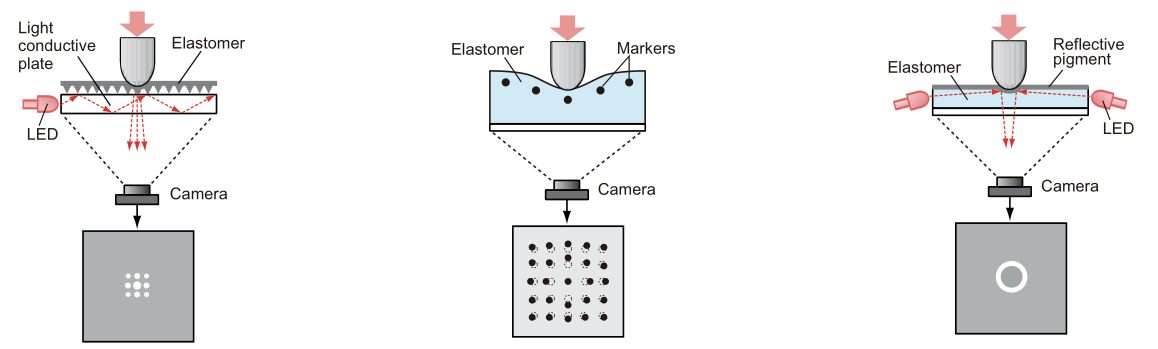
\includegraphics[width=\textwidth]{optical-tactile-sensors.png}
		\caption{Types of optical-based tactile sensors: Light conductive plate, Marker displacement, Reflective membrane (from left to right) \cite{shimonomura2019tactile}.}
	\end{figure}
	\item Strain gauges
	\item Audio-based tactile sensors: can provide information about surface texture.
	\item Multi-component tactile sensors
\end{itemize}
Prior works use tactile sensors in inference of object properties \cite{luo2017robotic} and robotic manipulation \cite{yamaguchi2019recent}.
\begin{itemize}
	\item Grasping
	\begin{itemize}
		\item Heuristic grasp adaptation strategy
		\item Grasp adaptation with slip detection
		\item Grasp adaptation with estimating friction coefficient
		\item Grasp adaptation with grasp stability estimation
		\item Complete grasp process with tactile sensing
	\end{itemize}
	\item Other robotic manipulation
	\begin{itemize}
		\item Detecting events with tactile sensors
		\item Estimating pose and location with tactile sensors
		\item Reinforcement learning with tactile sensors
		\item Exploring the workspace without vision
	\end{itemize}
	\item Tactile perception
\end{itemize}

Issues of introducing tactile sensors to robotic hands:
\begin{itemize}
	\item Difficulty to install on robotic hands.
	\item Wiring, power supply, and processing.
	\item Low durability, fragility.
	\item Less compatibility with the other tactile sensors.
	\item It is unclear what we can do with tactile sensors.
	\item Disadvantages caused by tactile sensors.
	\begin{itemize}
		\item Maintenance becomes complicated.
		\item Programming becomes complicated.
	\end{itemize}	
	\item Expensive.
	\item Asking for the moon.
\end{itemize}

\section{Data Acquisition \& Sensor Fusion}

\section{Signal Preprocessing}

\section{Communication \& Signal Transmission}
\subsection{Challenges in Data Transmission}
\begin{itemize}
	\item Different forms (text, speech, images)
	\item Large distances, limited time
	\item Certain bandwidth
\end{itemize}

\subsection{Information Systems \& Data Transmission Principles}
\subsection{Transmission Media}
\subsection{Network Topologies \& Data Transmission Protocols}
Topologies: $\begin{matrix*}[l]
	- \text{P2P}\\
	- \text{Bus}\\
	- \text{Fieldbus}
\end{matrix*}$

Protocols: OSI and TCP/IP

\subsection{Robot Communication with ROS}